\documentclass[border=0pt]{standalone}
\usepackage{amsmath}
\usepackage[usenames,dvipsnames]{xcolor}
\usepackage{graphicx}

%%font
\usepackage{euler}
\usepackage[OT1]{eulervm}
\renewcommand{\rmdefault}{pplx}

\usepackage{tikz}
\tikzset{roundnode/.style={circle,draw=black,fill=blue!20}}
\definecolor{TortugaColor}{rgb}{0.1,0.4,0.3}
\definecolor{Totemblue}{HTML}{09182F}
\definecolor{Totemred}{HTML}{2B030B}
\definecolor{Totemyellow}{HTML}{AD901B}
\usetikzlibrary{intersections}
%\usetikzlibrary{fadings}
\usetikzlibrary{arrows}
%\usetikzlibrary{arrows.meta}
%\usetikzlibrary{decorations}
\usetikzlibrary{decorations.pathmorphing}
\usetikzlibrary{decorations.text}
%\usetikzlibrary{fit}
%\usetikzlibrary{calc}
%\usetikzlibrary{through}
%\usetikzlibrary{positioning}
%\usetikzlibrary{graphs}
%\usetikzlibrary{mindmap}
%\usetikzlibrary{backgrounds}
%\usetikzlibrary{calligraphy}
\usepgfmodule{nonlineartransformations}
\usetikzlibrary{curvilinear}

%%% Set up polar step (code from the pgd manual)
%\makeatletter
%\def\polartransformation{%
% \pgf@x will contain the radius
% \pgf@y will contain the distance
%\pgfmathsincos@{\pgf@sys@tonumber\pgf@x}%
% pgfmathresultx is now the cosine of radius and
% pgfmathresulty is the sine of radius
%\pgf@x=\pgfmathresultx\pgf@y%
%\pgf@y=\pgfmathresulty\pgf@y%
%}
%\makeatother

\pgfdeclarelayer{background}
\pgfdeclarelayer{alpha}
\pgfdeclarelayer{beta}
\pgfsetlayers{background,alpha,main,beta}

%%pic TaiJi
\tikzset{
TaiJi/.pic={
\begin{scope}[thick,yi/.style={radius=0.4cm}]
\shade [draw=black] (0,0) circle [radius =3];
\shade [top color=black, bottom color=black!50,draw=black] (0,-3) arc [radius=3, start angle=-90, end angle=90]
arc [radius=1.5, start angle=90, end angle=270]
arc [radius=1.5, start angle=90, end angle=-90];
\draw[thin,fill=black] (0,-1.5) circle [yi];
\draw[thin,fill=white] (0,1.5) circle [yi];
\end{scope}
}}

%%pic Totu
\tikzset{
totu/.pic={
\begin{scope}[scale=0.2]
\pgfmathsetmacro{\legwidth}{0.4*0.2}
\draw[fill=green!60!black!30] (0,0.8) circle [x radius=0.3,y radius=0.4];
\foreach \i in {-1,1}{
\begin{scope}[xscale=\i]
\path (0.8,0) edge[draw=green!60!black!30,line width=\legwidth cm,line cap=round,bend left] ++(0.6,0);
\path (0.6,-1) edge[draw=green!60!black!30,line width=\legwidth cm,line cap=round] ++ (0.4,-0.4);
\end{scope}
}
\draw (0,-1.4) edge[draw=green!60!black!30,line width=\legwidth cm,line cap=round] ++ (0,-0.4);
\draw[fill=green!60!black,rounded corners] (1,0) -- (0,0.5) -- (-1,0) -- (-0.8,-1.2) -- (0,-1.6) -- (0.8,-1.2) -- cycle;
\end{scope}
}}

%%pic Rescuer
\tikzset{
Rescuer/.pic={
\begin{scope}[shift={(6.35,1.2)}]
\draw[fill=black!20!red!60!yellow] (-7,-0.8) -- (-6.7,-1.2) -- (-6,-1.2) -- (-5.7,-0.8) .. controls +(-0.3,-0.1) and +(0.3,-0.1) ..  cycle;
\end{scope}
}}

%%pic SatanHeart
\tikzset{
SatanHeart/.pic={
\pgfmathsetmacro{\SatanHradius}{1}
\pgfmathsetmacro{\LSatanHradius}{1.05}
\begin{scope}[very thick]
\draw[gray!80!blue, line width=2pt] (0,0) circle[radius=\LSatanHradius cm];
\draw[gray!80!blue] (-90:\SatanHradius) -- (-306:\SatanHradius) -- (-162:\SatanHradius) -- (-378:\SatanHradius) -- (-234:\SatanHradius) -- cycle;
\end{scope}
}}

%%pic Stone Gate
\tikzset{
stonegate/.pic={
\begin{scope}[gray]
\draw[fill,draw=none,rounded corners] (-1.3,-0.3) rectangle (-0.7,2);
\draw[fill,draw=none,rounded corners] (0.7,-0.3) rectangle (1.3,2);
\draw[fill,draw=none] (0,2) ellipse[x radius=2cm, y radius=0.3cm];
\end{scope}
}}
 
%%pic Ateles Zombia
\tikzset{
zombia/.pic={
\pgfmathsetmacro{\zombiascale}{0.2}
\begin{scope}[scale=\zombiascale]
\pgfmathsetmacro{\zombiawidth}{\zombiascale *0.3 cm}
\pgfmathsetmacro{\zombiabigcorner}{\zombiascale *4 pt}
\pgfmathsetmacro{\zombiasmallcorner}{\zombiascale *0.2 cm}
\begin{scope}[gray!40, rounded corners=\zombiabigcorner, line width=\zombiawidth, line cap=round]
%\node[circle,draw,thin] at (0,0) {};
\draw [fill,thin] (-1.9,0.4) circle [radius=0.3cm];
\draw (-1.8,0.1) -- (-2.2,-0.3) -- (-2.7,-0.6);
\draw (-1.8,0.1) -- (-1.6,-0.8) -- ++ (0.1,-0.1);
\draw (-1.8,0.1) -- (-0.9,0.1) -- (0.4,0.8);
\draw[rounded corners=\zombiasmallcorner] (0.4,0.8) -- ++ (0.3,0.2) -- ++ (0.2,-0.2);
\draw (0.7,1) -- (0.9,1.3) -- (1,2.5) -- (1.3,3) -- (1.8,2.9);
\draw (0.9,0.8) -- (0.9,0.5) -- (0.95,-0.3) -- (0.8,-1.1);
\draw (0.8,0.8) -- (0.4,0.6) -- (0,-0.7) -- ++(-0.2,-0.2);
\end{scope}
\end{scope}
}
}

%%pic family
\tikzset{
family/.pic={
\begin{scope}[xshift=-1cm]
\clip (0,0) rectangle (2,1);
\draw[fill] (0.25,0.7) circle [radius=0.1cm];
\draw[line cap=round,line width=0.06cm] (0.25,0.7) -- (0.25,0.2);
\draw[line cap=round,line width=0.06cm] (0.15,0) -- (0.25,0.2) -- (0.35,0);

\draw[fill] (0.75,0.6) circle [radius=0.1cm];
\draw[line cap=round,line width=0.06cm] (0.75,0.6) -- (0.75,0.2);
\draw[line cap=round,line width=0.06cm] (0.65,0) -- (0.75,0.2) -- (0.85,0);

\draw[fill] (1.25,0.6) circle [radius=0.1cm];
\draw[line cap=round,line width=0.06cm] (1.25,0.6) -- (1.25,0.2);
\draw[line cap=round,line width=0.06cm] (1.15,0) -- (1.25,0.2) -- (1.35,0);

\draw[fill] (1.75,0.65) circle [radius=0.1cm];
\draw[line cap=round,line width=0.06cm] (1.75,0.65) -- (1.75,0.2);
\draw[line cap=round,line width=0.06cm] (1.65,0) -- (1.75,0.2) -- (1.85,0);

\draw[line cap=round, line width=0.06cm] (0,0.3) -- (0.25,0.5) -- (0.5,0.3) -- (0.75,0.4) -- (1,0.3) -- (1.25,0.4) -- (1.5,0.3) -- (1.75,0.45) -- (2,0.3);
\end{scope}
}
}

\parindent=0pt

\begin{document}
%%2020NewYear
%% 16:9
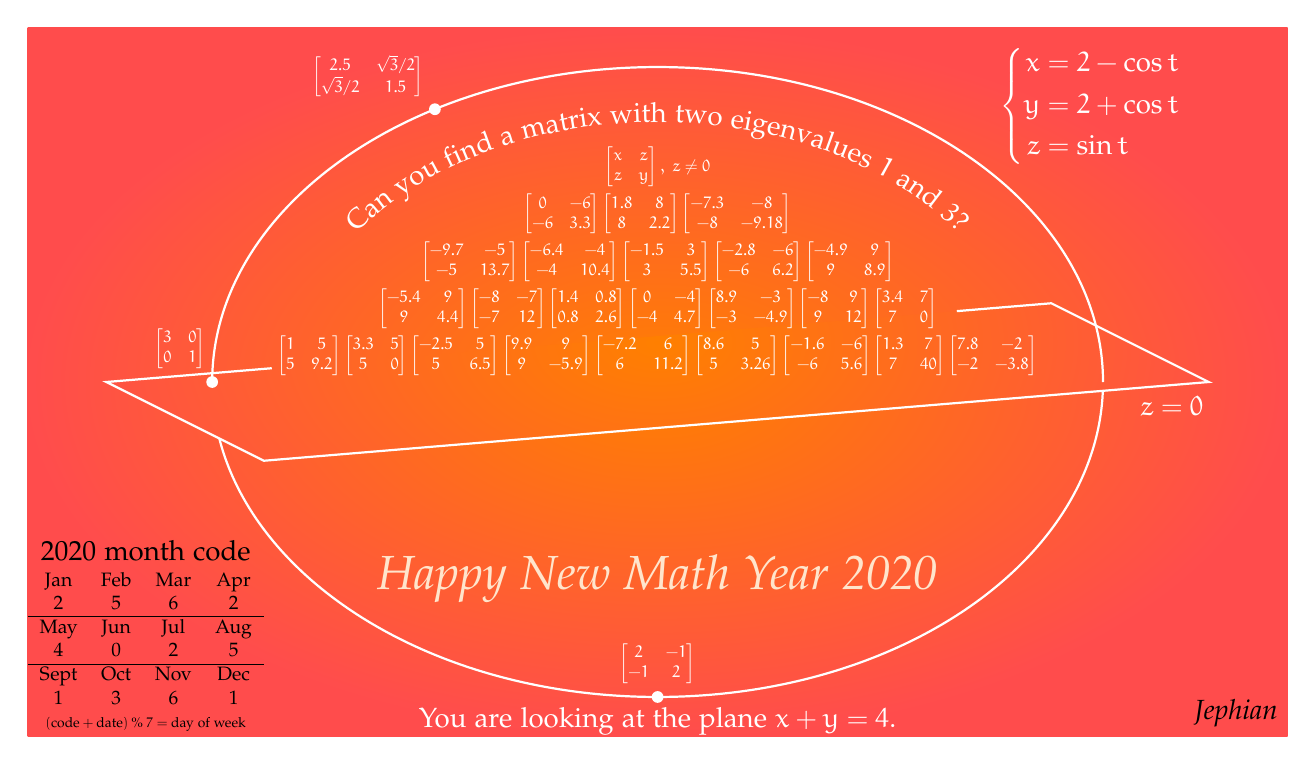
\begin{tikzpicture}
\coordinate (Jamaica) at (-8,-4);
\coordinate (Dominican) at (8,-4);
\coordinate (Cuba) at (-8,5);
\coordinate (TurksCaicos) at (8,5);
\coordinate (Tortuga) at (0,0);
\clip (Jamaica) rectangle (TurksCaicos);

%%Help Lines
\begin{pgfonlayer}{beta}
%\draw [step=1, black!50, thin] (Jamaica) grid (TurksCaicos);
%\draw (0,0) circle [radius=0.2cm];
\end{pgfonlayer}

%%background Layer
\begin{pgfonlayer}{background}
\shade [inner color=orange, outer color=red!70] (-8,-4) rectangle (8,5);
\end{pgfonlayer} 


%%Main Layer (main)
\begin{pgfonlayer}{main}

%%% start yshift=0.5cm
\begin{scope}[white, thick, yshift=0.5cm]

%%% Iso-spectral manifold and Pattern manifold
\coordinate (m13) at (5.6568,0);
\coordinate (m31) at (-5.6568,0);

%%% lower iso-spectral
\draw[thick] (m31) arc (180:360:5.6568cm and 4cm);

%%% pattern
\begin{scope}
\clip (-7,0) -- ++(2,-1) -- (7,0) -- ++ (-2,1) -- cycle;
\shade[inner color=orange, outer color=red!70] (-8,-4) rectangle (8,5);
\end{scope}
\draw (-4.9,0.175) -- (-7,0) -- ++(2,-1) -- (7,0) -- ++ (-2,1) -- ++(-1.2,-0.1);

%%% upper iso-spectral
\draw (m13) arc (0:180:5.6568cm and 4cm);

%%% Haystack of matrices
%%% Layer 1
\node[rectangle,draw=none,above,scale=0.6,transform shape] at (0,0) {$
\begin{bmatrix}
1 & 5 \\
5 & 9.2 \\
\end{bmatrix}
\begin{bmatrix}
3.3 & 5 \\
5 & 0 \\
\end{bmatrix}
\begin{bmatrix}
-2.5 & 5 \\
5 & 6.5 \\
\end{bmatrix}
\begin{bmatrix}
9.9 & 9 \\
9 & -5.9 \\
\end{bmatrix}
\begin{bmatrix}
-7.2 & 6 \\
6 & 11.2 \\
\end{bmatrix}
\begin{bmatrix}
8.6 & 5 \\
5 & 3.26 \\
\end{bmatrix}
\begin{bmatrix}
-1.6 & -6 \\
-6 & 5.6 \\
\end{bmatrix}
\begin{bmatrix}
1.3 & 7 \\
7 & 40 \\
\end{bmatrix}
\begin{bmatrix}
7.8 & -2 \\
-2 & -3.8 \\
\end{bmatrix}
$};
%%% Layer 2
\node[rectangle,draw=none,above,scale=0.6,transform shape] at (0,0.6) {$
\begin{bmatrix}
-5.4 & 9 \\
9 & 4.4 \\
\end{bmatrix}
\begin{bmatrix}
-8 & -7 \\
-7 & 12 \\
\end{bmatrix}
\begin{bmatrix}
1.4 & 0.8 \\
0.8 & 2.6 \\
\end{bmatrix}
\begin{bmatrix}
0 & -4 \\
-4 & 4.7 \\
\end{bmatrix}
\begin{bmatrix}
8.9 & -3 \\
-3 & -4.9 \\
\end{bmatrix}
\begin{bmatrix}
-8 & 9 \\
9 & 12 \\
\end{bmatrix}
\begin{bmatrix}
3.4 & 7 \\
7 & 0 \\
\end{bmatrix}
$};
%%% Layer 3
\node[rectangle,draw=none,above,scale=0.6,transform shape] at (0,1.2) {$
\begin{bmatrix}
-9.7 & -5 \\
-5 & 13.7 \\
\end{bmatrix}
\begin{bmatrix}
-6.4 & -4 \\
-4 & 10.4 \\
\end{bmatrix}
\begin{bmatrix}
-1.5 & 3 \\
3 & 5.5 \\
\end{bmatrix}
\begin{bmatrix}
-2.8 & -6 \\
-6 & 6.2 \\
\end{bmatrix}
\begin{bmatrix}
-4.9 & 9 \\
9 & 8.9 \\
\end{bmatrix}
$};
%%% Layer 4
\node[rectangle,draw=none,above,scale=0.6,transform shape] at (0,1.8) {$
\begin{bmatrix}
0 & -6 \\
-6 & 3.3 \\
\end{bmatrix}
\begin{bmatrix}
1.8 & 8 \\
8 & 2.2 \\
\end{bmatrix}
\begin{bmatrix}
-7.3 & -8 \\
-8 & -9.18 \\
\end{bmatrix}
$};
%%% Layer 5
\node[rectangle,draw=none,above,scale=0.6,transform shape] at (0,2.4) {$
\begin{bmatrix}
x & z \\
z & y \\
\end{bmatrix},
\ z\neq 0
$};

%%Find a matrix
\draw[decorate,decoration={text along path,text={|\color{white}|Can you find a matrix with two eigenvalues $1$ and $3$?}}] (145:4.667cm and 3.3cm) arc (145:35:4.667cm and 3.3cm);

%% z = 0
\node[rectangle, draw=none, right] at (6,-0.3) {$z=0$};

%% x + y = 4
\node[rectangle, draw=none, below] at (0,-4) {You are looking at the plane $x + y = 4$.};

%% Parametrization
\node[rectangle, draw=none] at ([shift={(-2.5,-1)}]TurksCaicos) {$
\left\{\begin{aligned}
x &= 2 - \cos t \\
y &= 2 + \cos t \\
z &= \sin t
\end{aligned}\right.
$};

%% Three points
\node[circle, fill, draw=none, inner sep=1.5pt, label={[scale=0.6]above:$\begin{bmatrix}2&-1\\-1&2\end{bmatrix}$}] at (270:5.6568cm and 4cm) {};
\node[circle, fill, draw=none, inner sep=1.5pt, label={[scale=0.6]95:$\begin{bmatrix}3&0\\0&1\end{bmatrix}$}] at (180:5.6568cm and 4cm) {};
\node[circle, fill, draw=none, inner sep=1.5pt, label={[scale=0.6]135:$\begin{bmatrix}2.5&\sqrt{3}/2\\\sqrt{3}/2&1.5\end{bmatrix}$}] at (120:5.6568cm and 4cm) {};

\end{scope}
%%% start yshift=0.5cm


\end{pgfonlayer}


%%beta layer
\begin{pgfonlayer}{beta}

%%Happy New Math Year
%\draw[decorate,decoration={text along path,text={|\color{red!80!yellow} \LARGE \it|Happy New Math Year 2020}}] (-3.5,-2.5) .. controls (-1,4.5) and (1,4.5) .. (3.5,-2.5);
\node[rectangle, draw=none, red!50!yellow!20] at (0,-2) {\LARGE\it Happy New Math Year 2020};

\node[rectangle, draw=none, opacity=0] at (0,-0.5) {\Huge\tt FREE HONG KONG};

%%Month code
\node[above] at (-6.5,-1.9) {2020 month code};
\node[scale=0.7,below] at (-6.5,-1.8) {\begin{tabular}{cccc} 
Jan & Feb & Mar & Apr \\
 2 & 5 & 6 & 2 \\
\hline
May & Jun & Jul & Aug \\
 4 & 0 & 2 & 5 \\
\hline
Sept & Oct & Nov & Dec \\
 1 & 3 & 6 & 1 \\
\end{tabular}};
\node[scale=0.5,above] at (-6.5,-4) {$(\text{code}+\text{date})\mathbin{\%}7=\text{day of week}$};

%%Signature
\node[yshift=0.3cm,left] at (Dominican) {\it Jephian};

\end{pgfonlayer}




\end{tikzpicture}
\end{document}


%%\draw=\path[draw]
%%\clip=\path[clip]
%%\graph=\path[graph]
%%bend right ~ bend right=30 ~ in,out=right30, left 30
%%(left:2)=(180:2)
%%left ~ anchor=east ~ anchor 0
%%for sharp corners: line cap, line joint
%%for elliptical rectangle: smooth circle, plot coordinates, tensions
%For updating 2.10 to 3.0.0
%after moving the folder, it requires 
%sudo texhash 
% to make it work.
%%To convert to jpg: compile the pdf first, and then use the command below
%% convert -density 300 file.pdf -quality 90 file.jpg
%% required to install imagemagick

%% use pdf2png in AUR with Resolution 500 for 2018 
%% use gimp for 2019 (resolution 1890 x 1062, export quality 90)

%% Sample transformation as below
\makeatletter
\def\mytrans{
    \pgfmathparse{\pgf@x+1cm}
    %\pgf@x=\pgfmathresult pt
    \pgfmathsetlength{\pgf@x}{\pgfmathresult pt}
}
\makeatother










%%%%% code for generating matrices

def latex_matrix(A):
    m,n = A.dimensions();
    print(r"\begin{bmatrix}")
    for i in range(m):
        print(' & '.join([('%.2f'%num).rstrip('0').rstrip('.') for num in A[i]]) + r' \\')
    print(r"\end{bmatrix}")

small = [k/10 for k in range(-99,100)]
small_int_no0 = list(range(-9,10))
small_int_no0.remove(0)

def ram_mtx():
    again = True
    while again:
        again = False
        ### mode 0: trace = 4
        ### mode 1: det = 3
        ### mode 3: no restrictions
        mode = choice([0]*6 + [1]*2 + [2]*2)
        M = zero_matrix(QQ,2,2)
        M[0,0] = choice(small)
        M[0,1] = choice(small_int_no0)
        M[1,0] = M[0,1]
        if mode == 0:
            M[1,1] = 4 - M[0,0]
        if mode == 1:
            M[1,1] = N((3 + M[1,0]*M[0,1]) / M[0,0])
        if mode == 2:
            M[1,1] = choice(small)
        if M.trace() == 4 and M.determinant() == 3:
            again = True
    return M

for _ in range(3):
    M = ram_mtx()
    latex_matrix(M)

A = matrix(QQ, [
    [1.4,0.8],
    [0.8,2.6]
])
latex_matrix(A)
